\chapter{Effects of Social Constraints}
Each of the proposed social constraints in this thesis has some particular effect on the behaviour of the robot. Some of the predominant effects of these are briefly presented here. Each case presents a scenario without and with the social constraint activated. The figures of each scenario show the paths taken by the human and the robot (starting at blue and moving towards red) and their velocities (robot's velocity in red and human's velocity in blue) below. The velocity plot also includes the distance between the human and the robot during the execution of the scenario. 

\section{TTCplus Constraint}
\subsection{Approach}
\begin{figure}[!htb]
\centering
\begin{subfigure}{0.5\columnwidth}
  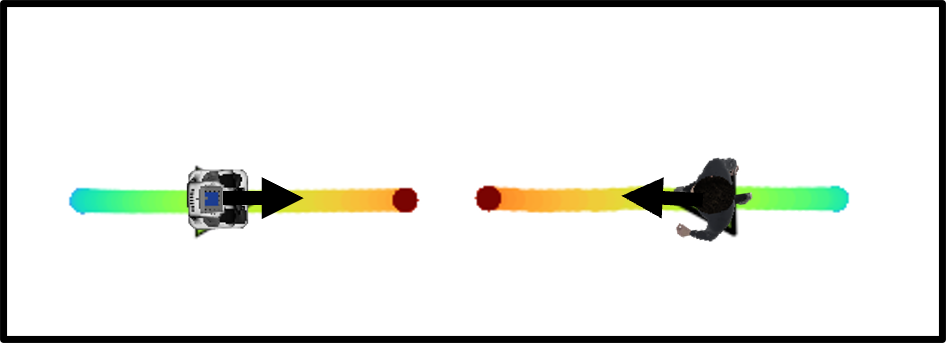
\includegraphics[width=\textwidth]{images/appendix/ttc/approach/approach_without.png}
\end{subfigure}
\vspace{0.5cm}
\begin{subfigure}{0.8\columnwidth}
  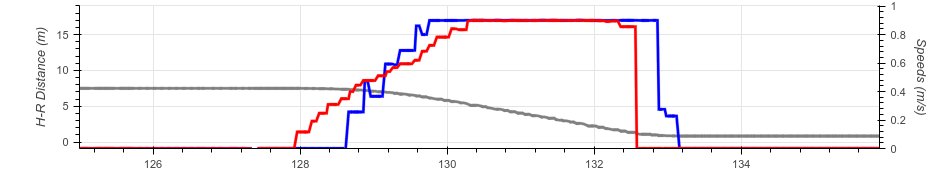
\includegraphics[width=\textwidth]{images/appendix/ttc/approach/without.png}
  \caption{without TTCplus}
\end{subfigure}

\begin{subfigure}{0.5\columnwidth}
  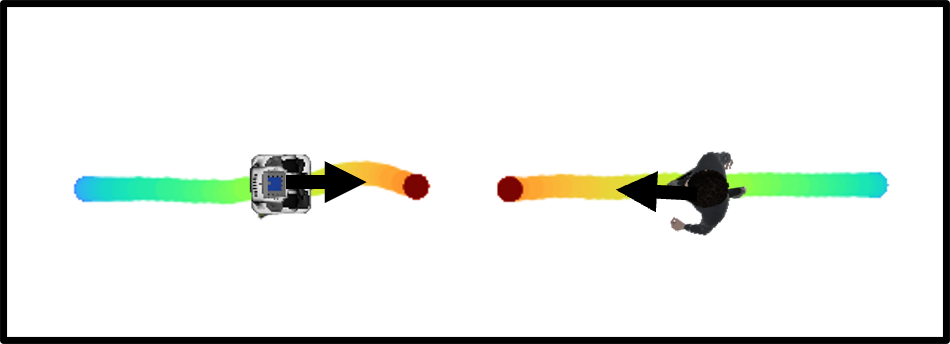
\includegraphics[width=\textwidth]{images/appendix/ttc/approach/approach_with.png}
\end{subfigure}
% \hspace{-0.75cm}
\begin{subfigure}{0.8\columnwidth}
  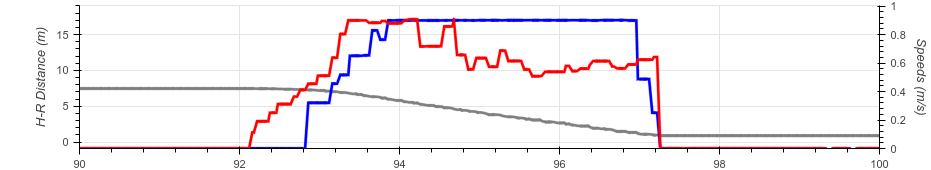
\includegraphics[width=\textwidth]{images/appendix/ttc/approach/with1.png}
  \caption{with TTCplus}
\end{subfigure}
\caption{The robot approaches a human head-on. The addition of the TTCplus constraint makes the robot deviate a little and slow down as it nears the human.}
\label{fig:approach_ttc}
\end{figure} 

In this scenario, the robot and human move towards each other and stop at a very close distance from each other. From Fig.~\ref{fig:approach_ttc} (a), it can be seen that the robot and human move at their full speeds towards each. However, with the addition of the TTCplus constraint, the robot has a decreasing velocity profile as the human-robot distance decreases, showing the robot's intention to stop (shown in Fig.~\ref{fig:approach_ttc} (b)).

\subsection{Open Space Crossing}
\begin{figure}[H]
\centering
\begin{subfigure}{0.5\columnwidth}
  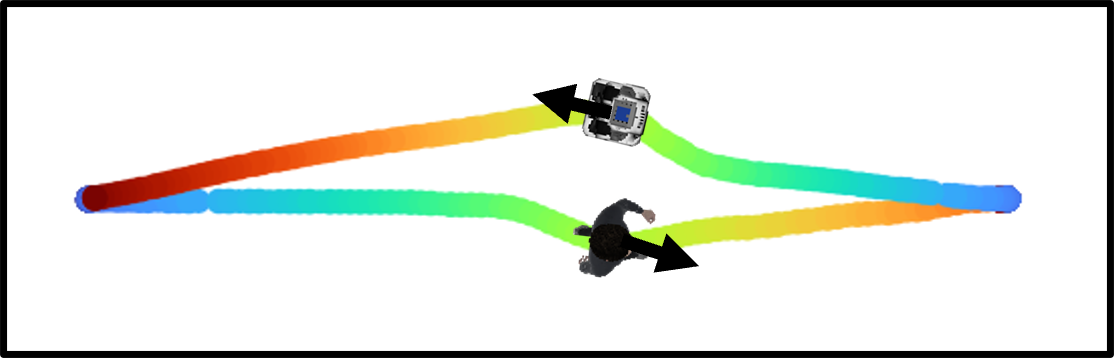
\includegraphics[width=\textwidth]{images/appendix/ttc/wide/without.png}
\end{subfigure}
\vspace{0.5cm}
\begin{subfigure}{0.8\columnwidth}
  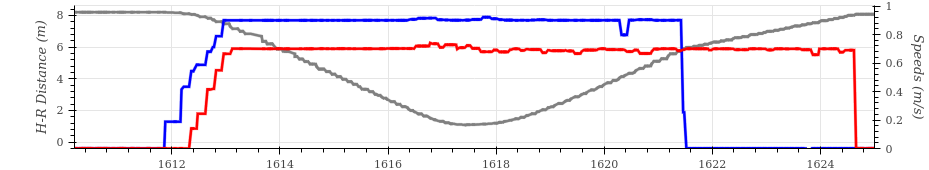
\includegraphics[width=\textwidth]{images/appendix/ttc/wide/wide_without1.png}
  \caption{without}
\end{subfigure}

\begin{subfigure}{0.5\columnwidth}
  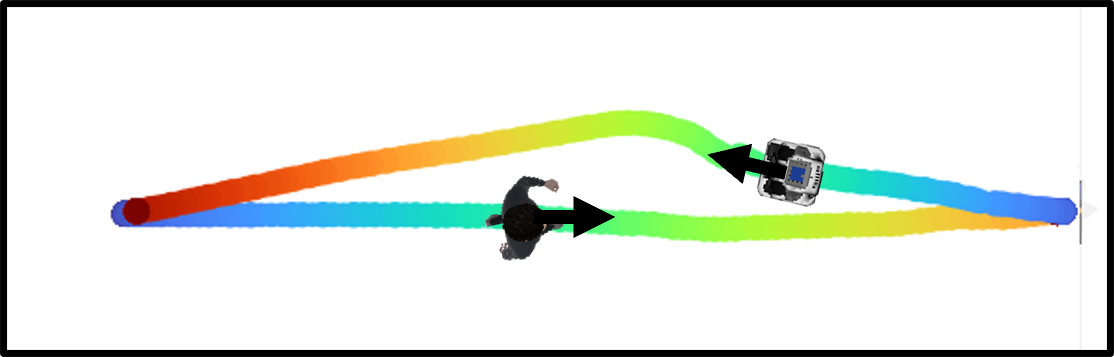
\includegraphics[width=\textwidth]{images/appendix/ttc/wide/with.png}
\end{subfigure}
% \hspace{-0.75cm}
\begin{subfigure}{0.8\columnwidth}
  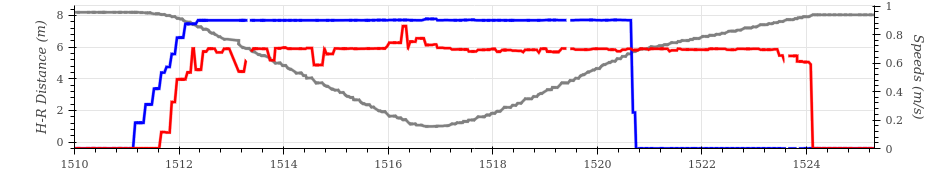
\includegraphics[width=\textwidth]{images/appendix/ttc/wide/wide_with2.png}
  \caption{with}
\end{subfigure}
\caption{The human and the robot cross each other in an open space. The addition of the TTCplus constraint makes the robot move aside quickly, showing its intention to give way and the choice of its side to move.}
\label{fig:open_space_ttc}
\end{figure} 

\hspace{\parindent} This scenario simulates a robot crossing a human in an open area where there is enough space to move away and not disturb the human. In Fig.~\ref{fig:open_space_ttc} (a), the robot and human move directly towards each other and only avoid each other at the last minute before the collision. This puts on an additional burden on the human to deviate from his path to avoid a collision with the robot. A more human-aware robot should avoid the occurrence of such path deviation, which is similar to what is seen in Fig.~\ref{fig:open_space_ttc} (b). Therefore, the TTCplus constraint not only shows its intention to move away early but also reduces the additional navigational burden that might be imposed on the human.  

\subsection{Corridor Crossing}
\begin{figure}[H]
\centering
\begin{subfigure}{0.5\columnwidth}
  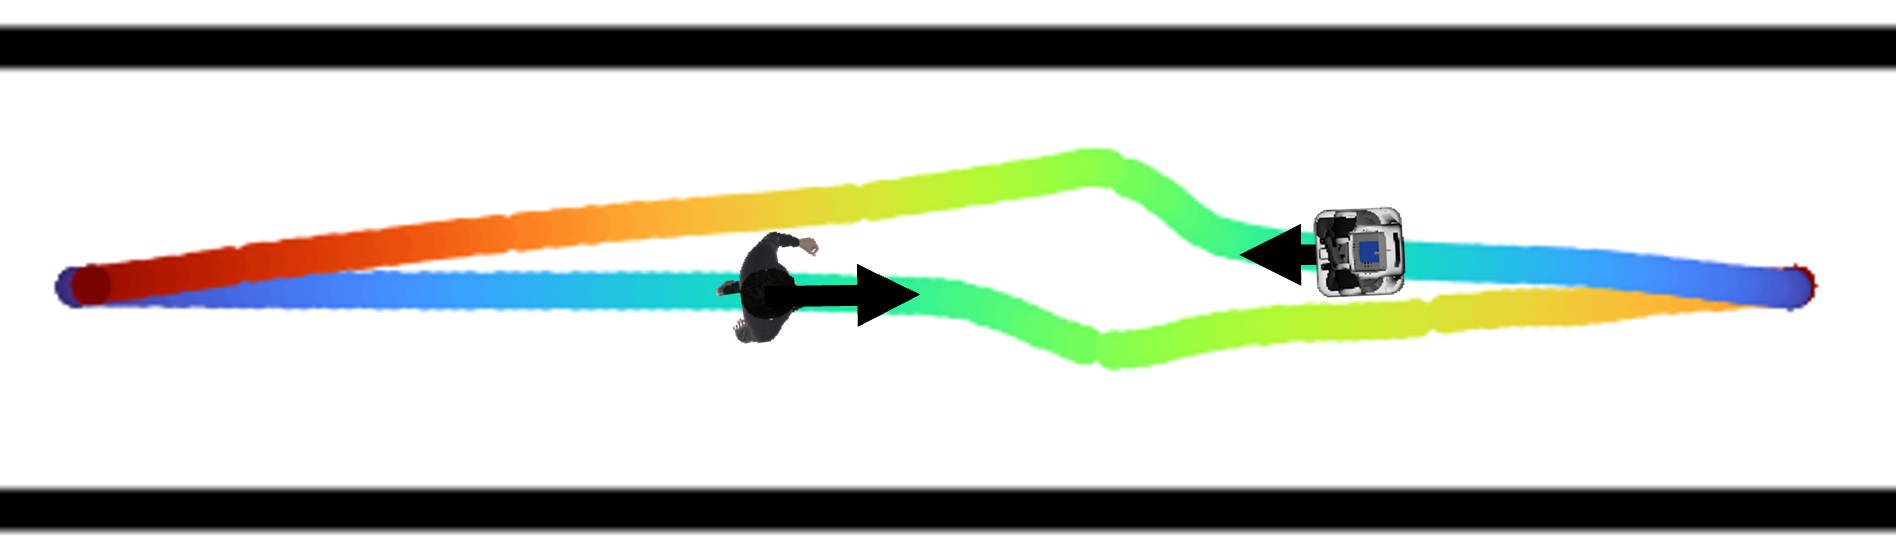
\includegraphics[width=\textwidth]{images/appendix/ttc/corridor/without.png}
\end{subfigure}
\vspace{0.5cm}
\begin{subfigure}{0.8\columnwidth}
  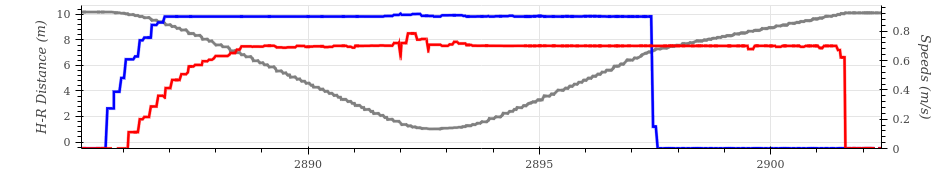
\includegraphics[width=\textwidth]{images/appendix/ttc/corridor/coor_without2.png}
  \caption{without}
\end{subfigure}

\begin{subfigure}{0.5\columnwidth}
  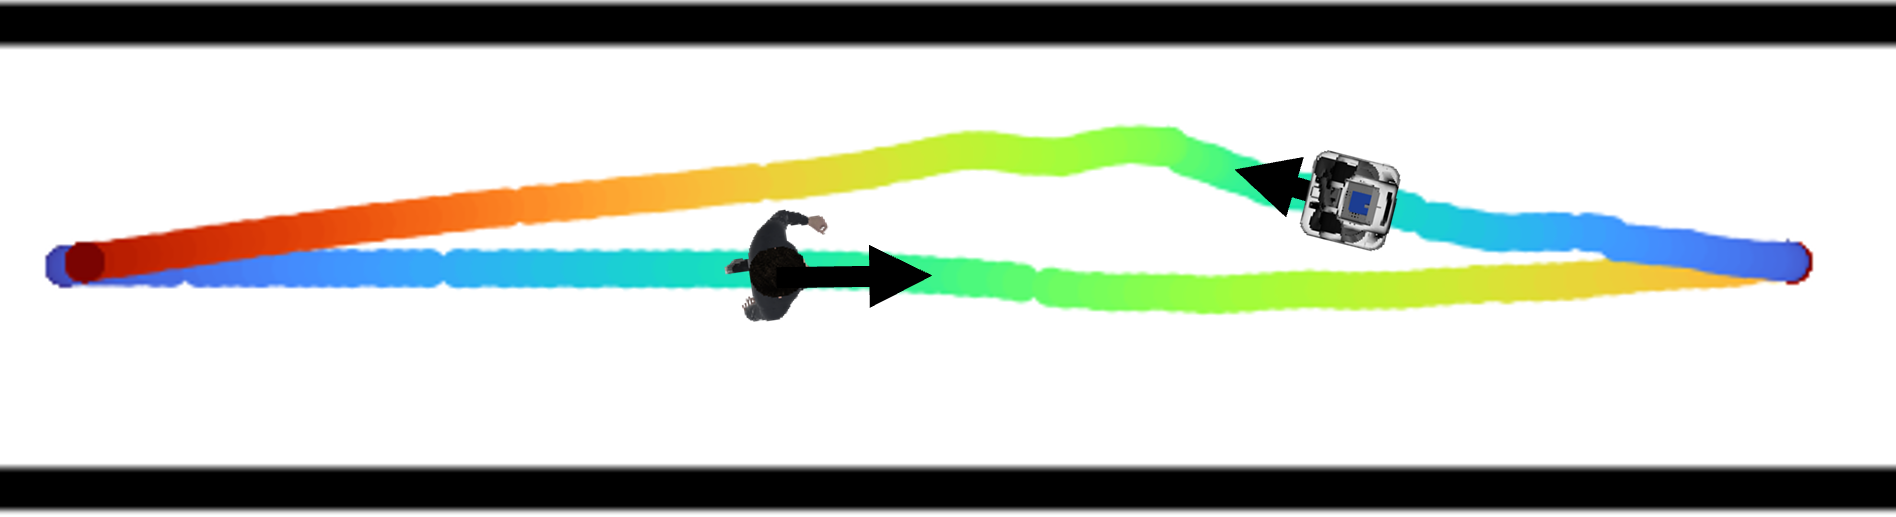
\includegraphics[width=\textwidth]{images/appendix/ttc/corridor/with.png}
\end{subfigure}
% \hspace{-0.75cm}
\begin{subfigure}{0.8\columnwidth}
  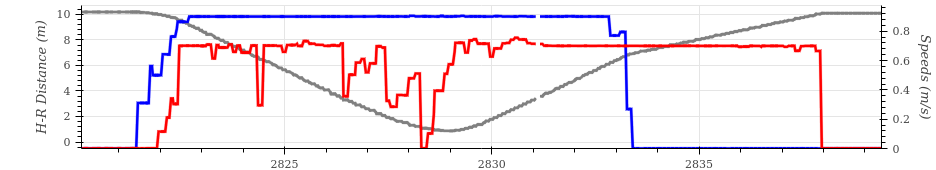
\includegraphics[width=\textwidth]{images/appendix/ttc/corridor/coor_with2.png}
  \caption{with}
\end{subfigure}
\caption{The human and the robot cross each other in a corridor. TTCplus constraint not only makes the robot take a side early but also slows down the robot as it crosses the human.}
\label{fig:corridor_ttc}
\end{figure} 

\hspace{\parindent} This scenario is similar to the previous one, but the space is narrower. As there is not enough space to move away, the robot with the TTCplus constraint moves to a side as well as slows down, as shown in Fig.~\ref{fig:corridor_ttc} (b). Without this constraint, it behaves exactly like in the previous case (Fig.~\ref{fig:corridor_ttc} (a)). 

\section{Relative Velocity Constraint}
\subsection{Corridor Crossing}
\hspace{\parindent} The corridor crossing scenario is the same as the one shown in the previous section. In the case of the Relative Velocity constraint, the robot should try to move away as quickly as possible and provide more space for the human even when the line of travel is not the same. This can be clearly seen from the path and the velocity profile of the robot in Fig.~\ref{fig:corridor_rel}. The robot starts to move to one side very quickly and slows down as it crosses the human. If there was enough space, the robot could have moved with a larger velocity while crossing. This constraint addresses parallel travel better when compared to TTCplus.

\begin{figure}[H]
\centering
% \begin{subfigure}{0.4\columnwidth}
%   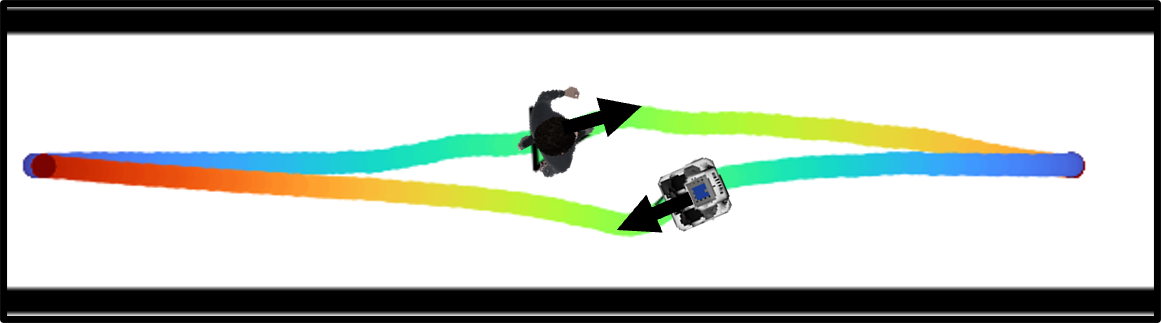
\includegraphics[width=\textwidth]{images/appendix/relvel/corridor/without.png}
% \end{subfigure}
% \vspace{0.5cm}
% \begin{subfigure}{0.8\columnwidth}
%   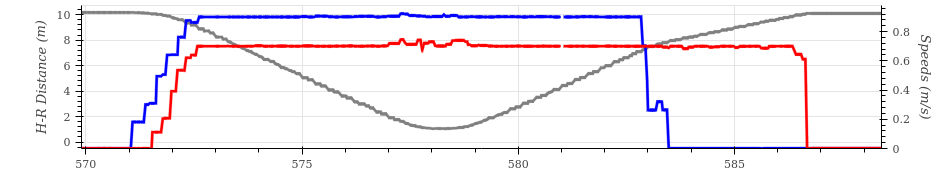
\includegraphics[width=\textwidth]{images/appendix/relvel/corridor/corr_without2.png}
%   \caption{without}
% \end{subfigure}

\begin{subfigure}{0.5\columnwidth}
  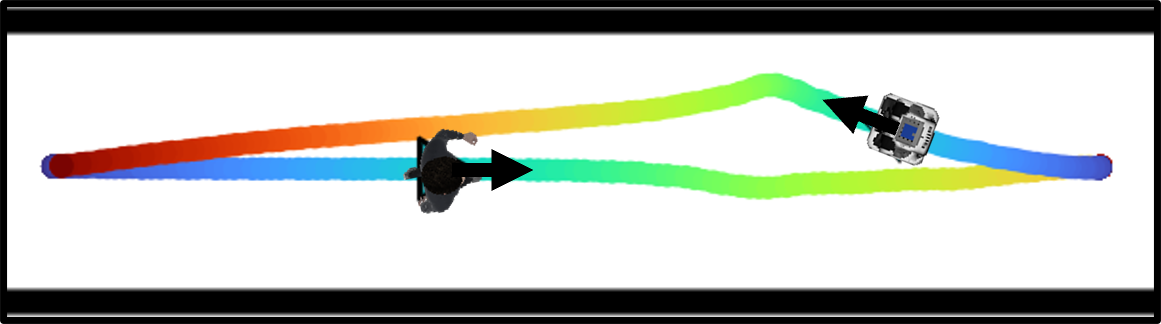
\includegraphics[width=\textwidth]{images/appendix/relvel/corridor/with.png}
\end{subfigure}
% \hspace{-0.75cm}
\begin{subfigure}{0.8\columnwidth}
  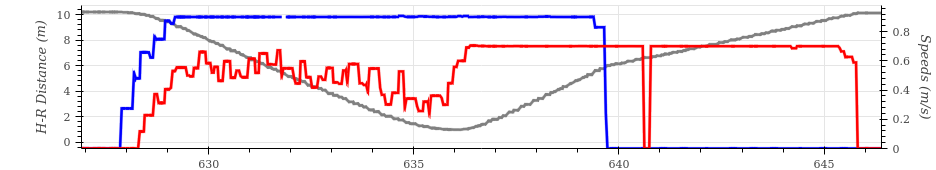
\includegraphics[width=\textwidth]{images/appendix/relvel/corridor/corr_with2.png}
  % \caption{with Relative Velocity Constraint}
\end{subfigure}
\caption{The human and the robot cross each other in a corridor. Relative Velocity constraint makes the robot clear the way quickly and move with a slower speed robot as it crosses the human at a small parallel distance.}
\label{fig:corridor_rel}
\end{figure} 

\subsection{Open Space Crossing}

\begin{figure}[H]
\centering
% \begin{subfigure}{0.4\columnwidth}
%   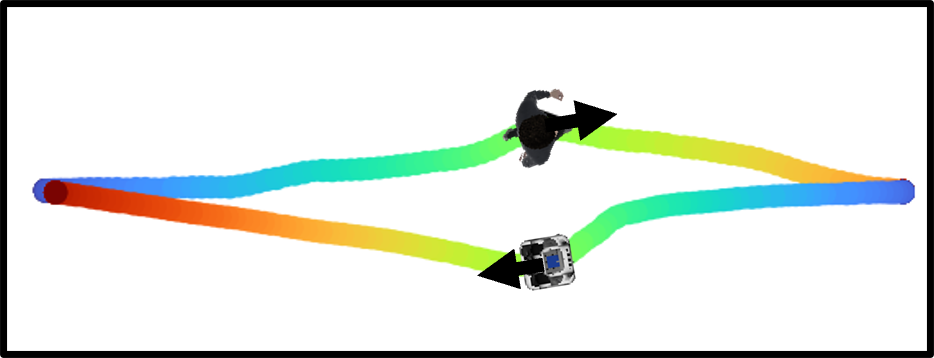
\includegraphics[width=\textwidth]{images/appendix/relvel/wide/without.png}
% \end{subfigure}
% \vspace{0.5cm}
% \begin{subfigure}{0.8\columnwidth}
%   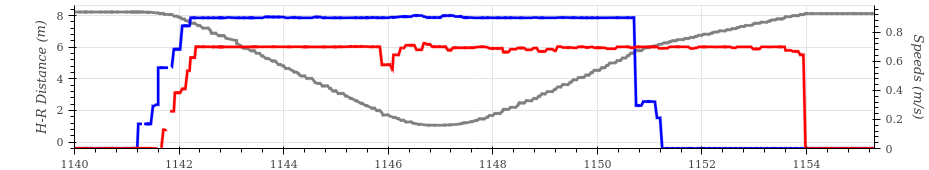
\includegraphics[width=\textwidth]{images/appendix/relvel/wide/without2.png}
%   \caption{without}
% \end{subfigure}

\begin{subfigure}{0.5\columnwidth}
  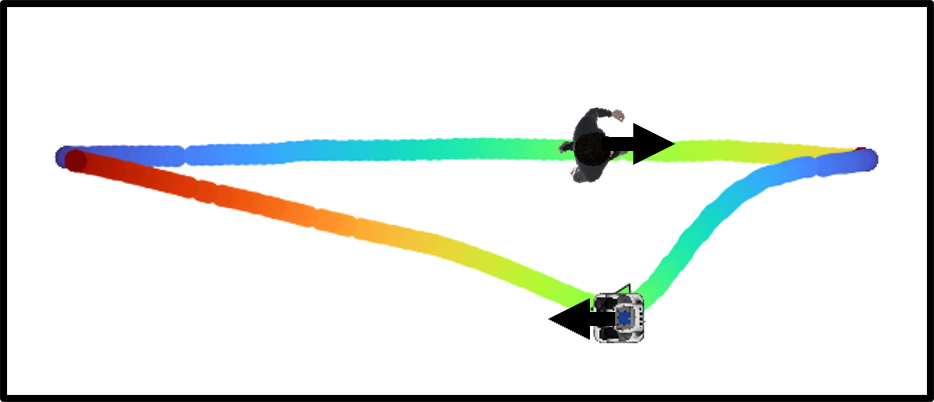
\includegraphics[width=\textwidth]{images/appendix/relvel/wide/with.png}
\end{subfigure}
% \hspace{-0.75cm}
\begin{subfigure}{0.8\columnwidth}
  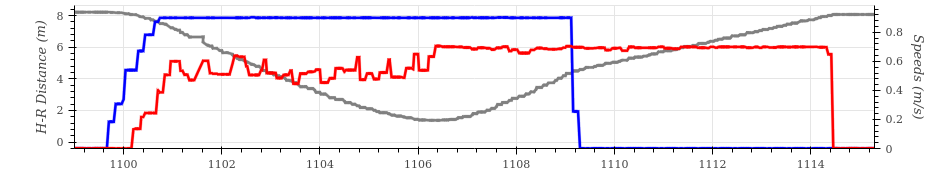
\includegraphics[width=\textwidth]{images/appendix/relvel/wide/with2.png}
  % \caption{with}
\end{subfigure}
\caption{The human and the robot cross each other in an open space. The addition of the Relative Velocity constraint makes the robot take a large deviation by exploiting the available space while showing its intention to give way. It also facilitates the robot to move at a larger velocity towards the goal.}
\label{fig:wide_rel}
\end{figure}

\hspace{\parindent} In this setting, the robot has enough space to move away and then travel with a larger velocity. Without the addition of the Relative Velocity constraint, the robot and human avoid each other moments before the collision, similar to Fig.~\ref{fig:open_space_ttc} (a). This constraint makes the robot move away very quickly and exploit the available space to move at full speed towards its goal. It can be observed from the path and the speed profile of the robot in Fig.~\ref{fig:wide_rel}. This clearly shows how the Relative Velocity constraint addresses the parallel travel better compared to the TTCplus constraint (see Fig.~\ref{fig:open_space_ttc} (b)).

\section{Visibility Constraint}
\hspace{\parindent} To show the advantage of adding the visibility constraint, an overtaking scenario is simulated. In this setting, the robot encounters a human moving very slowly and partially blocking its way. The robot has to over the human in order to move to its goal faster. In the first case, shown in Fig.~\ref{fig:visib_const} (a), without the addition of Visibility constraint, the robot overtakes the human very closely and also disturbs his navigation. With the addition of this constraint, however, the robot takes a large deviation and tries to enter the human's field of view as far as possible without disturbing him. This can be observed from the plots in Fig.~\ref{fig:visib_const} (b).
\begin{figure}[H]
\centering
\begin{subfigure}{0.5\columnwidth}
  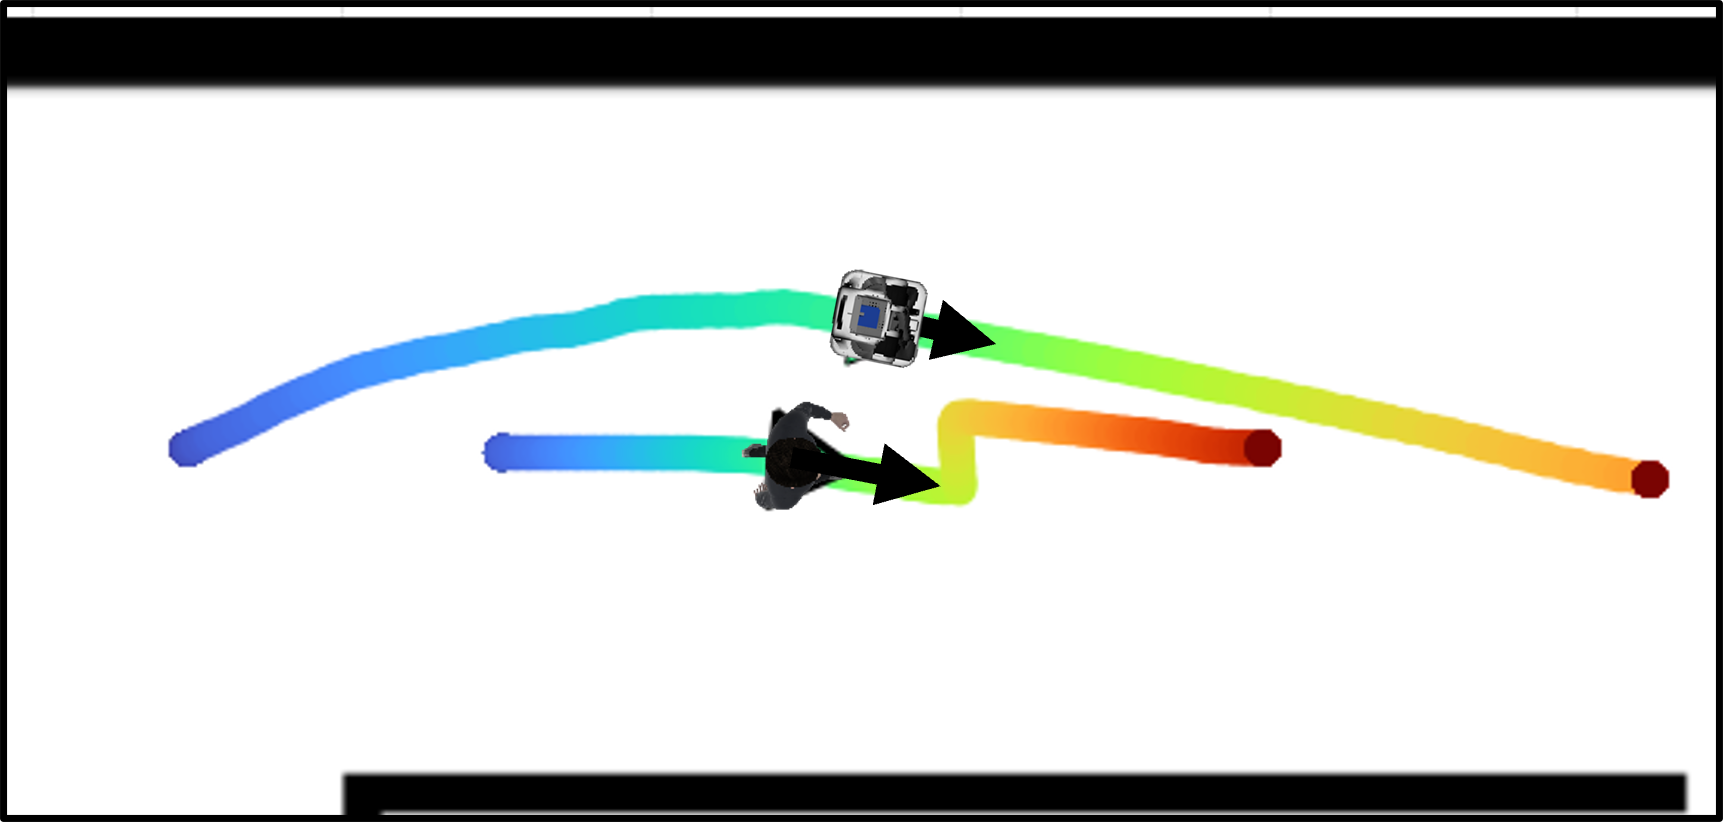
\includegraphics[width=\textwidth]{images/appendix/vis/without.png}
\end{subfigure}
\vspace{0.5cm}
\begin{subfigure}{0.8\columnwidth}
  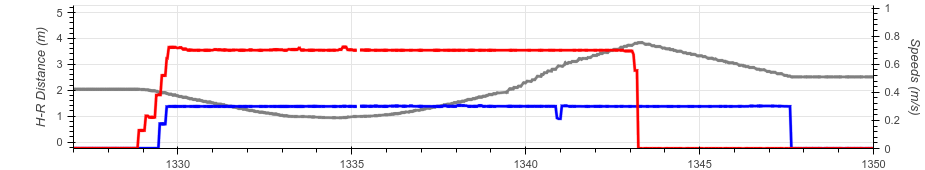
\includegraphics[width=\textwidth]{images/appendix/vis/without1.png}
  \caption{without}
\end{subfigure}

\begin{subfigure}{0.5\columnwidth}
  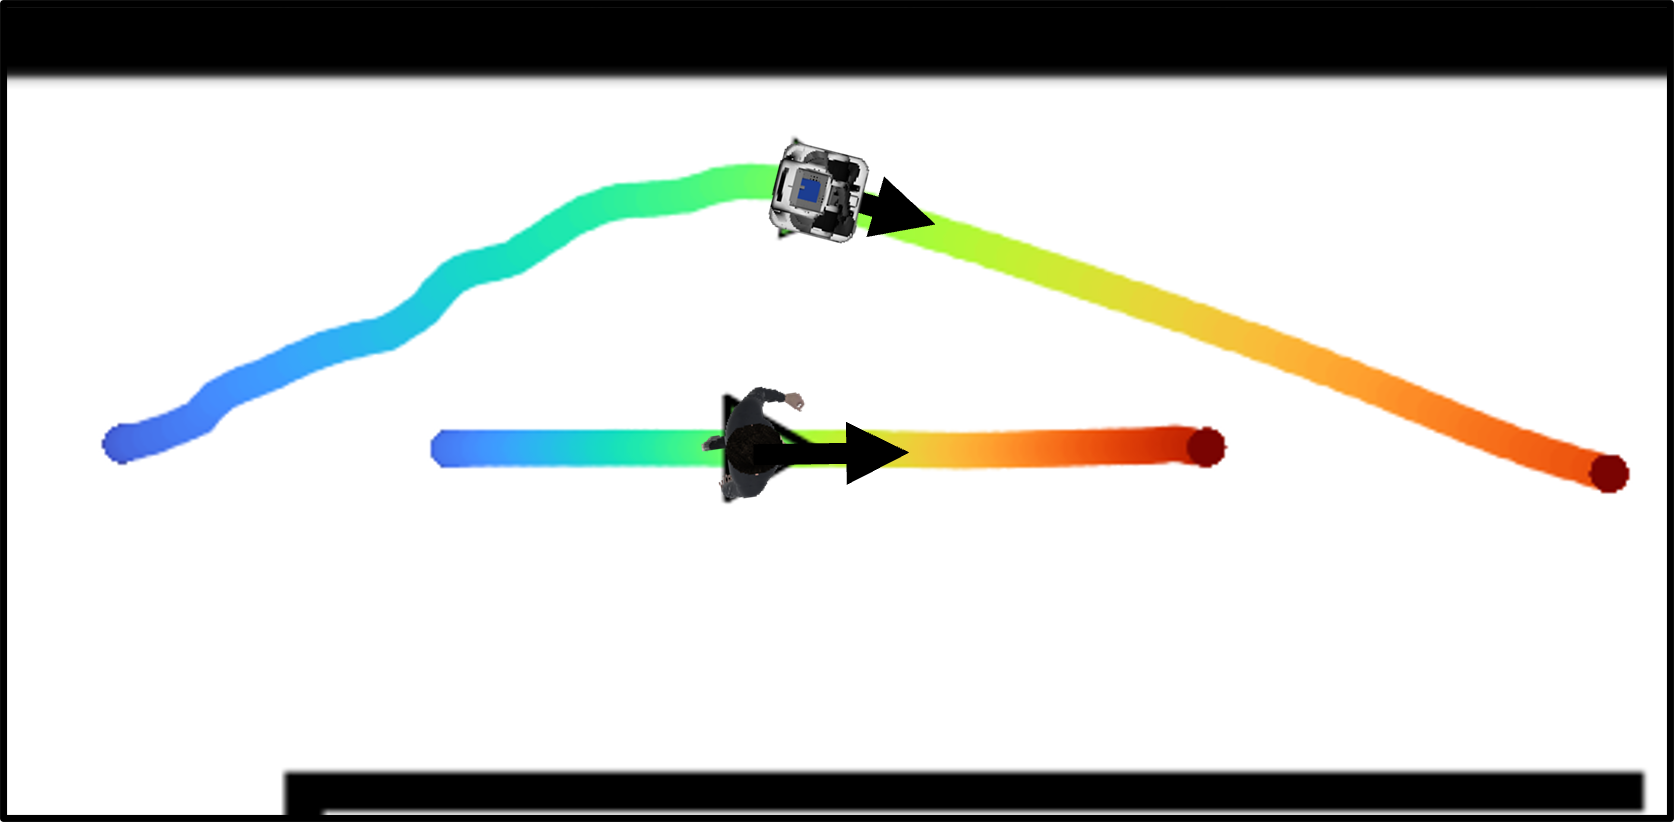
\includegraphics[width=\textwidth]{images/appendix/vis/with.png}
\end{subfigure}
% \hspace{-0.75cm}
\begin{subfigure}{0.8\columnwidth}
  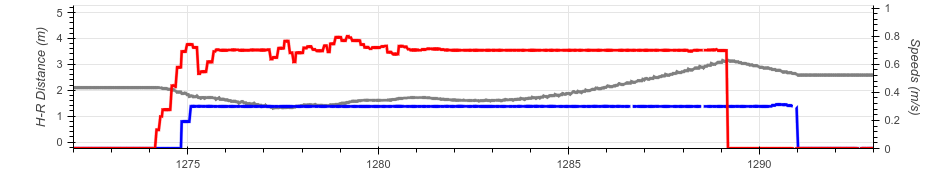
\includegraphics[width=\textwidth]{images/appendix/vis/with2.png}
  \caption{with}
\end{subfigure}
\caption{The robot overtakes a human who is moving very slowly. The addition of the Visibility constraint makes the robot enter the human's field of view slowly without surprising or disturbing the human.}
\label{fig:visib_const}
\end{figure}

\section{Updated Invisible Humans Constraint}
\hspace{\parindent} As shown in chapter~\ref{chap:5}, the current version of the `Invisible Humans' constraint already addresses a lot of scenarios to proactively accommodate sudden human appearances. However, the defined formulation had some issues which needed to be addressed using passage detection and mode shifting. After testing the robot navigation in more complicated scenarios, we observed that the current formulation could lead to some deadlocks even after the passage detection. One such deadlock situation is shown in Fig.~\ref{fig:inv_fail}. Here, the robot faces opposing forces from the obstacles and the invisible humans and freezes before it can even detect an opening.
\begin{figure}[h]
    \centering
    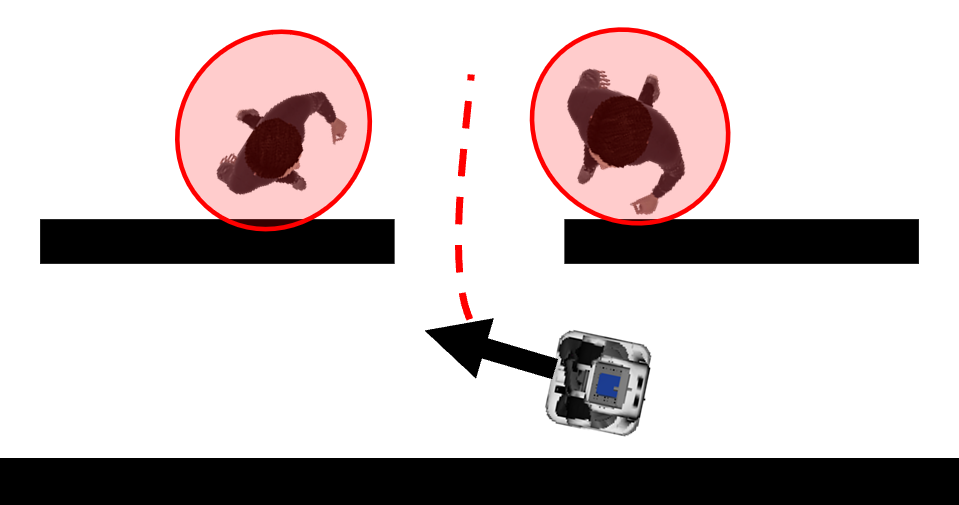
\includegraphics[width=0.8\columnwidth]{images/appendix/inv/updated_inv.png}
    \caption{A situation where the current formulation of the Invisible Humans constraint could fail. The opposing forces from the obstacles and the invisible humans make the robot freeze without moving.}
    \label{fig:inv_fail}
\end{figure}
Therefore, we update our formulation by taking inspiration from the Relative Velocity constraint. Instead of using the velocity of the visible humans, we use the defined invisible humans' velocity in the formulation and update the formulation as follows:
\begin{equation}
\begin{split}
cost_{inv\_human} &= max\left(\frac{V-a\Delta t_n+\lVert\overrightarrow{V_r}\rVert+1}{d}, 0\right)\quad \text{if}\quad \Delta t_n> 0.5s\\
                &= \frac{V}{d}\quad otherwise
\end{split}
\label{updated_inv_eq}
\end{equation}

In the latest version of CoHAN, the above formulation is used instead of the previous one. The rigorous testing of the updated formulation is still pending, but we already see some improvements over the previous one. An example of the constrained door crossing is presented below.

\subsection{Testing the Updated Constraint}
\hspace{\parindent} The above formulation acts on the robot's velocity during the possible freezing scenarios and makes the robot move with lower velocities, and reduces the cost. Since it is an updated formulation of the Invisible Humans constraint, it should still hold the properties of the previous formulation. To show this, we have simulated the door crossing scenario again with a wall on the side that limits the space. 

In Fig.~\ref{fig:door_inv_new} (a), the robot moves without considering and accounting for the invisible humans in the environment. Therefore, it moves at almost full speed and takes the shortest path to reach the goal. With the formulation in chapter~\ref{chap:5}, the robot froze between the wall and the entry to the door and did not move. However, with the updated formulation, the robot moves away from the door as much as possible without colliding with the wall and also aligns itself to properly pass through the door. Further, while crossing the door, the robot moves very cautiously with a slower velocity, as seen in Fig.~\ref{fig:door_inv_new} (b) between $140-145 s$.
\begin{figure}[!ht]
\centering
\begin{subfigure}{0.3\columnwidth}
  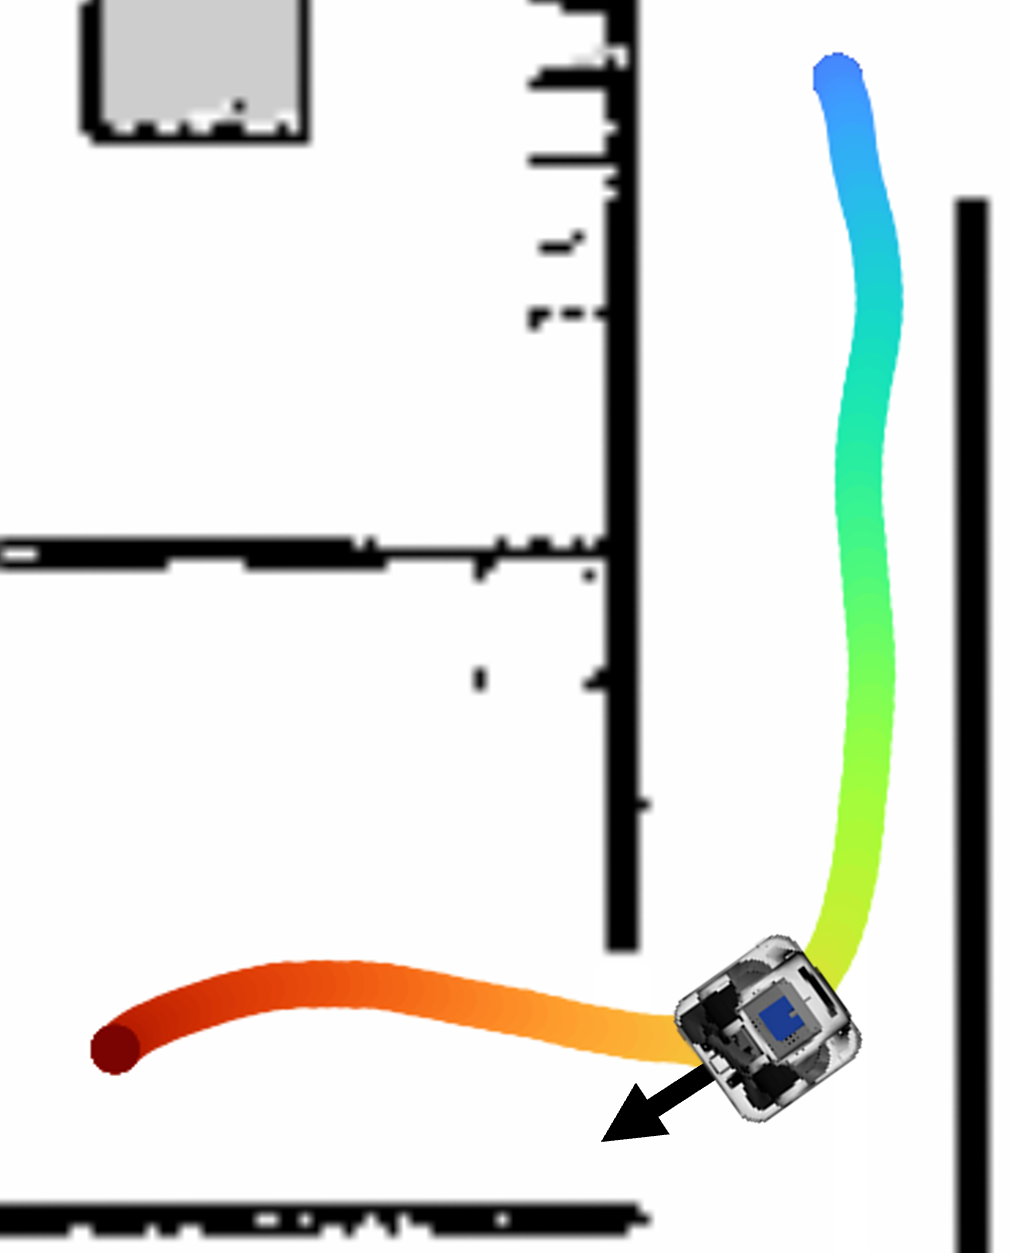
\includegraphics[width=\textwidth]{images/appendix/inv/without.png}
\end{subfigure}
\vspace{0.5cm}
\begin{subfigure}{0.8\columnwidth}
  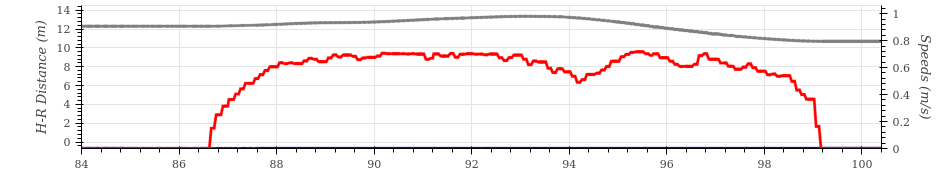
\includegraphics[width=\textwidth]{images/appendix/inv/without2.png}
  \caption{Without Invisible Humans constraint}
\end{subfigure}

\begin{subfigure}{0.3\columnwidth}
  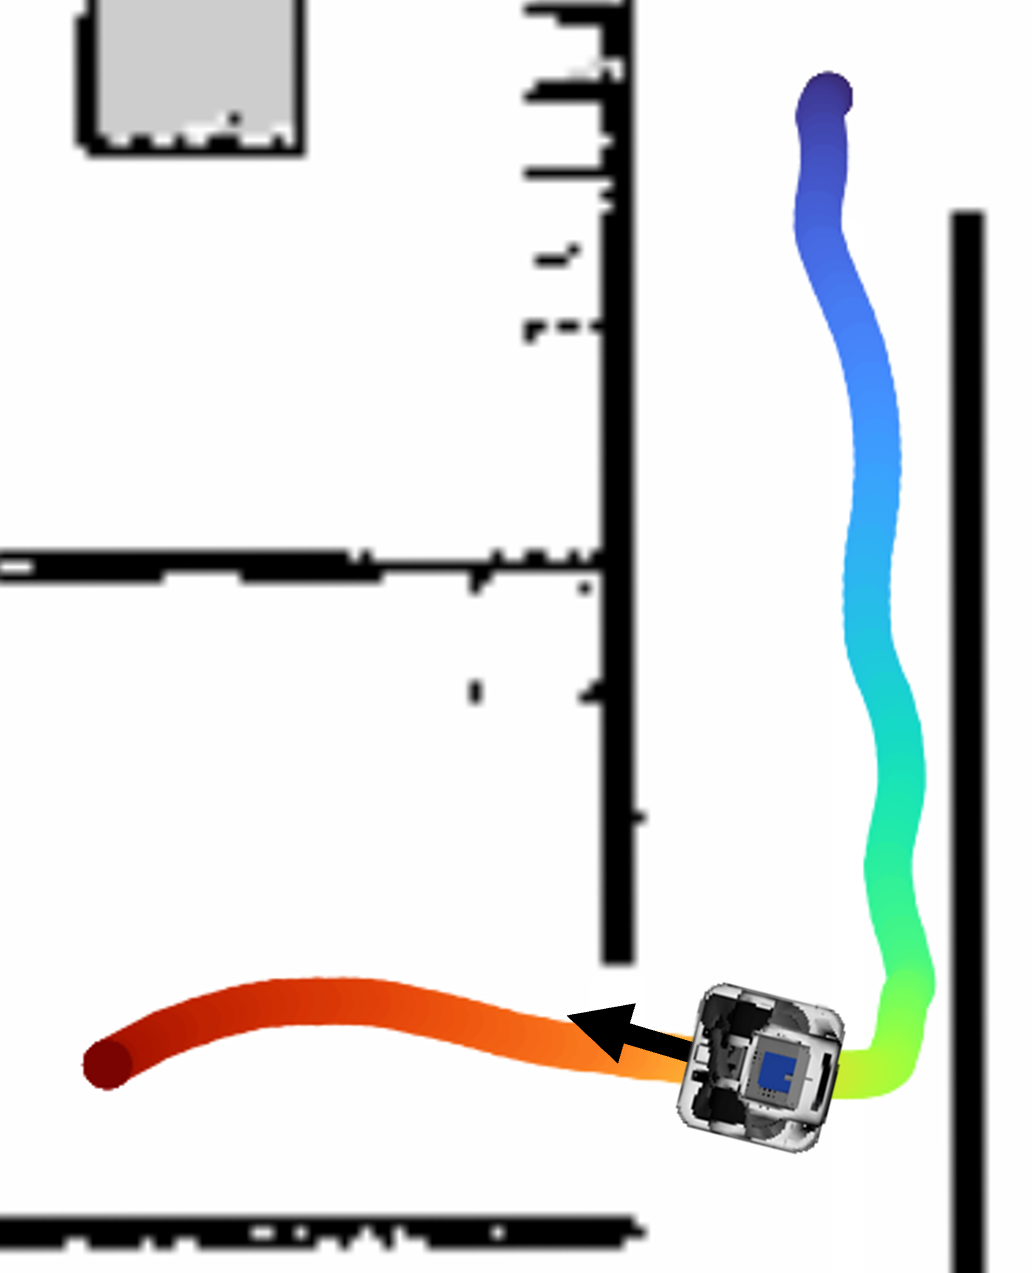
\includegraphics[width=\textwidth]{images/appendix/inv/with.png}
\end{subfigure}
% \hspace{-0.75cm}
\begin{subfigure}{0.8\columnwidth}
  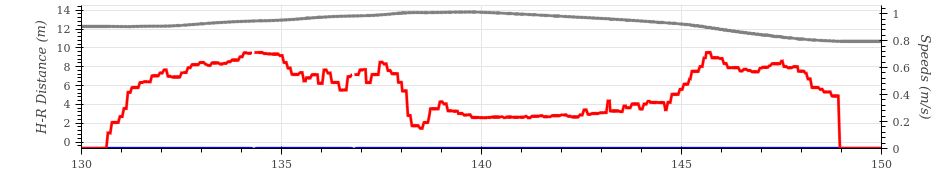
\includegraphics[width=\textwidth]{images/appendix/inv/with2.png}
  \caption{with the updated Invisible Humans constraint}
\end{subfigure}
\caption{Constrained door crossing scenario. The robot has to enter a door in a narrow space and try to accommodate humans as much as possible. The updated Invisible Humans constraint makes the robot move close to the wall before aligning itself towards the door and carefully entering it.}
\label{fig:door_inv_new}
\end{figure}